
%(BEGIN_QUESTION)
% Copyright 2011, Tony R. Kuphaldt, released under the Creative Commons Attribution License (v 1.0)
% This means you may do almost anything with this work of mine, so long as you give me proper credit

An operator notices that both pumps are running while level indicator LIR-134 shows a very low level in the sump (less than one foot):

$$\includegraphics[width=15.5cm]{i0005rx01.eps}$$

The operator summons you to investigate the problem.  What do you recommend as your first diagnostic test?

\vskip 20pt \vbox{\hrule \hbox{\strut \vrule{} {\bf Suggestions for Socratic discussion} \vrule} \hrule}

\begin{itemize}
\item{} What type of level-measurement technology is being used in this system?
\end{itemize}

\underbar{file i03528}
%(END_QUESTION)





%(BEGIN_ANSWER)

The first thing you should try to do is verify whether or not there is a real low-level condition in the tank.  If so, a danger exists in that the sump pumps may become damaged by running dry, and the pumps should be manually turned off.  If not, it's a matter of determining why the level control system ``thinks'' a high-level condition exists.

%(END_ANSWER)





%(BEGIN_NOTES)

\filbreak \vskip 20pt \vbox{\hrule \hbox{\strut \vrule{} {\bf Virtual Troubleshooting} \vrule} \hrule}

\noindent
{\bf Predicting the effect of a given fault:} present each of the following faults to the students, one at a time, having them comment on all the effects each fault would produce.

\begin{itemize}
\item{} 
\item{} 
\item{} 
\end{itemize}


\vskip 10pt


\noindent
{\bf Identifying possible/impossible faults:} present symptoms to the students and then have them determine whether or not a series of suggested faults could account for all the symptoms, explaining {\it why} or {\it why not} for each proposed fault:

\begin{itemize}
\item{} Symptom: {\it LI-138 (bubbler) registers substantially higher than LI-134 (guided-wave radar)}
\item{} Purge flow set too high -- {\bf Yes}
\item{} LY-134 failed -- {\bf No}
\item{} Process vapor density too low -- {\bf Yes} (but unlikely)
\item{} Process liquid density too low -- {\bf No}
\item{} GWR probe fouled -- {\bf No}
\item{} Process liquid density too high -- {\bf Yes}
\item{} Excessive vapor pressure built up inside of sump -- {\bf Yes}
\item{} Steam flow through eductor P-405 too high -- {\bf No}
\item{} LSL-133 trip value set too low -- {\bf No}
\end{itemize}


\vskip 10pt


\noindent
{\bf Determining the utility of given diagnostic tests:} present symptoms to the students and then propose the following diagnostic tests one by one.  Students rate the value of each test, determining whether or not it would give useful information (i.e. tell us something we don't already know).  Students determine what different results for each test would indicate about the fault, if anything:

\begin{itemize}
\item{} Symptom: {\it }
\item{}  -- {\bf Yes/No}
\item{}  -- {\bf Yes/No}
\end{itemize}


\vskip 10pt


\noindent
{\bf Diagnosing a fault based on given symptoms:} imagine the compressed nitrogen gas tank runs out feeding the bubble tube for LT-138 in this system (don't reveal the fault to students!).  Present the operator's observation(s) to the students, have them consider possible faults and diagnostic strategies, and then tell them the results of tests they propose based on the following symptoms, until they have properly identified the nature and location of the fault:

\begin{itemize}
\item{} {\it LIR-134 reads 6 feet 2 inches and rising}
\item{} FI-133 (rotameter) registers no purge flow
\item{} PT-137 and PG-417 read zero line pressure
\item{} Neither pump P-407 or P-408 is running
\item{} LC-133 (PLC) is in ``Run'' mode
\end{itemize}

%INDEX% Measurement, level: troubleshooting
%INDEX% Process: oily water sump (realistic P&ID shown)

%(END_NOTES)

